\usepackage{xcolor}
\usepackage{afterpage}
\usepackage{pifont,mdframed}
\usepackage[bottom]{footmisc}
\usepackage{multicol}

\makeatletter
\gdef\this@inputfilename{input.txt}
\gdef\this@outputfilename{output.txt}
\makeatother

\newcommand{\inputfile}{\texttt{input.txt}}
\newcommand{\outputfile}{\texttt{output.txt}}

\newenvironment{warning}
  {\par\begin{mdframed}[linewidth=2pt,linecolor=gray]%
    \begin{list}{}{\leftmargin=1cm
                   \labelwidth=\leftmargin}\item[\Large\ding{43}]}
  {\end{list}\end{mdframed}\par}

William e Giorgio sono appena stati promossi a ispettori di sicurezza alla Scuola Internazionale di Alta Formazione (SIAF), la struttura che si trova a Volterra e che viene utilizzata per svolgere molti degli stage di allenamento dei Probabili Olimpici. Affinché la struttura possa essere adatta ad ospitare tanti giovani ragazzi e ragazze, è necessario che le norme di sicurezza vengano rispettate alla lettera. Il direttore della SIAF ha quindi chiesto ai nuovi ispettori di aiutarlo ad analizzare la piantina della struttura in modo da trovare eventuali anomalie.

La richiesta del direttore è la seguente: viene data una mappa della SIAF in formato testuale, in cui le stanze (carattere \texttt{.}) sono delimitate dai muri (carattere \texttt{\#}) e possono contenere $0$ o più estintori (carattere \texttt{@}), ed è necessario capire in quali stanze \emph{non c'è} un estintore. Ad esempio, nella seguente mappa possiamo notare che ci sono $5$ stanze senza estintori:

\vspace{0.3cm}

\setlength\columnsep{50pt}

\begin{multicols}{2}
\hspace{1.0cm} 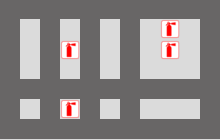
\includegraphics[width=0.85\linewidth]{map.png}

\begin{center}
{
\fontsize{1.0cm}{0.01em}
\begin{verbatim}
###########
#.#.#.#.@.#
#.#@#.#.@.#
#.#.#.#...#
###########
#.#@#.#...#
###########
\end{verbatim}
}
\end{center}

\end{multicols}

I muri della SIAF formano sempre una griglia, per cui le stanze sono tutte rettangolari. Quante stanze sono senza estintori?

\Implementation
Dovrai sottoporre esattamente un file con estensione \texttt{.c}, \texttt{.cpp} o \texttt{.pas}.

\begin{warning}
Tra gli allegati a questo task troverai un template (\texttt{estintori.c}, \texttt{estintori.cpp}, \texttt{estintori.pas}) con un esempio di implementazione da completare.
\end{warning}

Se sceglierai di utilizzare il template, dovrai implementare la seguente funzione:
\begin{center}\begin{tabularx}{\textwidth}{|c|X|}
\hline
C/C++  & \verb|int mancanti(int R, int C, char** M);|\\
\hline
Pascal & \verb|function mancanti(R, C: longint; var M: matrix): longint;|\\
\hline
\end{tabularx}\end{center}
In cui:
\begin{itemize}[nolistsep]
  \item Gli interi $R$ e $C$ rappresentano il numero di righe e colonne della mappa, rispettivamente.
  \item La matrice \texttt{M}, indicizzata da $0$ a $R-1$ sulle righe e da $0$ a $C-1$ sulle colonne, contiene i caratteri che descrivono la piantina dell'edificio.
  \item La funzione dovrà restituire il numero di stanze senza estintore, che verrà poi stampato sul file di output.
\end{itemize}

\InputFile
Il file \inputfile{} è composto da $R+1$ righe. La prima riga contiene due interi $R$ e $C$. Ognuna delle successive $R$ righe è lunga $C$ caratteri e descrive una riga della mappa.

\OutputFile
Il file \outputfile{} è composto da un'unica riga contenente un unico intero, il numero di stanze senza estintore.

% Assunzioni
\Constraints
\begin{itemize}[nolistsep, itemsep=2mm]
	\item $3 \le R, C \le 1000$.
    \item Ogni stanza è sempre composta da almeno un carattere \texttt{.} o un carattere \texttt{@}. In altre parole, non ci sono stanze ``schiacciate'' tra due muri adiacenti.
\end{itemize}

\Scoring
Il tuo programma verrà testato su diversi test case raggruppati in subtask.
Per ottenere il punteggio relativo ad un subtask, è necessario risolvere
correttamente tutti i test relativi ad esso.

\begin{itemize}[nolistsep,itemsep=2mm]
  \item \textbf{\makebox[2cm][l]{Subtask 1} [10 punti]}: Casi d'esempio.
  \item \textbf{\makebox[2cm][l]{Subtask 2} [20 punti]}: $R, C \le 30$.
  \item \textbf{\makebox[2cm][l]{Subtask 3} [40 punti]}: Tutte le stanze hanno zero estintori.
  \item \textbf{\makebox[2cm][l]{Subtask 4} [30 punti]}: Nessuna limitazione specifica.
\end{itemize}


\Examples
\begin{example}
\exmpfile{estintori.input0.txt}{estintori.output0.txt}%
\exmpfile{estintori.input1.txt}{estintori.output1.txt}%
\end{example}


\Explanation
Il \textbf{secondo caso di esempio} è lo stesso input che si trova nella figura nel testo.
